\chapter{Lipídios}\label{ch:b1:lipids}

Um camelo que atravessa um deserto carrega trinta quilos de \omterm{def:b1:lipids:triglyceride}{gordura} na
corcova e nenhuma água ali; uma truta num riacho de montanha a
\qty{4}{\celsius} tem membranas tão fluidas quanto as de uma carpa num
lago morno; e uma gota de azeite agitada em água se quebra numa nuvem de
gotículas que, deixadas em paz, tornam a se reunir numa só. As três
coisas são \omterm{def:b1:lipids:fattyacid}{lipídios} em ação: o estoque mais denso de energia química que
um \omterm{def:b1:organism-environment:organism}{organismo} consegue carregar, a película que delimita cada \omterm{def:b1:cell-unit-of-life:cell}{célula} e
cada organela, e a classe de moléculas que a água se recusa a
dissolver. Este capítulo descreve os \omterm{def:b1:lipids:fattyacid}{ácidos graxos} e as \omterm{def:b1:lipids:triglyceride}{gorduras}
construídas com eles, os \omterm{def:b1:lipids:fattyacid}{lipídios} \omterm{def:b1:lipids:amphiphilic}{anfifílicos} que se montam em
membranas, o que torna uma membrana mais ou menos fluida, e os outros
\omterm{def:b1:lipids:fattyacid}{lipídios} --- \omterm{def:b1:lipids:amphiphilic}{esteróis}, pigmentos, hormônios --- que alguns carbonos
arranjados em anéis e cadeias podem ser.

\section{Ácidos graxos}

\begin{definition}[Lipídio, ácido graxo]\label{def:b1:lipids:fattyacid}
Os \emph{lipídios}\index{lipídio} são as moléculas biológicas definidas
não por uma estrutura comum, e sim por uma propriedade comum: elas são
insolúveis em água e solúveis em solventes apolares. A maioria é
construída sobre \emph{ácidos graxos}\index{ácido graxo}: ácidos
carboxílicos com uma cadeia hidrocarbônica não ramificada de
\qtyrange{12}{24}{} carbonos, quase sempre em número par (eles são
montados de dois em dois carbonos,
\cref{ch:b1:biosyntheses-integration}). Um ácido graxo
\emph{saturado}\index{ácido graxo saturado} tem apenas ligações simples
e uma cadeia reta e flexível; um
\emph{insaturado}\index{ácido graxo insaturado} tem uma ou mais ligações
duplas, na configuração \emph{cis}, cada uma introduzindo na cadeia uma
dobra rígida de cerca de $30^\circ$. Notação: C18:1 $\Delta^9$ é um
ácido de 18 carbonos com uma ligação dupla depois do carbono 9 (o ácido
oleico); um ácido \emph{ômega-3} tem a última ligação dupla a três
carbonos da extremidade metila.
\end{definition}

\begin{omfigure}
\begin{tikzpicture}[font=\footnotesize, line cap=round, line join=round]
  % stearic acid: zig-zag of 18 carbons
  \draw[very thick, omDef!80!black] (0,0) \foreach \i in {1,...,17} { -- ++({0.36}, {0.22*(-1)^\i}) };
  \node[fill=omThm!25, draw=omThm, rounded corners=2pt, inner sep=2pt] at (-0.1,0.0) {COOH};
  \node[anchor=east, align=right] at (-0.85,0) {ácido esteárico C18:0\\ saturado, reto\\ funde a \qty{70}{\celsius}};
  \node[anchor=west] at (6.3,-0.22) {$\mathrm{CH_3}$};
  % oleic acid: kink at carbon 9-10, second half tilted downward
  \draw[very thick, omDef!80!black] (0,-2.0) \foreach \i in {1,...,8} { -- ++({0.36}, {0.22*(-1)^\i}) };
  \draw[very thick, omDef!80!black] (2.88,-2.0) -- ++(0.36,0.22);
  \draw[double, very thick, omThm] (3.24,-1.78) -- ++(0.36,0.22);
  \draw[very thick, omDef!80!black] (3.60,-1.56) \foreach \i in {1,...,8} { -- ++({0.33}, {0.22*(-1)^(\i+1)-0.13}) };
  \node[fill=omThm!25, draw=omThm, rounded corners=2pt, inner sep=2pt] at (-0.1,-2.0) {COOH};
  \node[anchor=east, align=right] at (-0.85,-2.0) {ácido oleico C18:1 $\Delta^9$\\ uma ligação dupla \emph{cis}, dobrado\\ funde a \qty{13}{\celsius}};
  \node[omThm, anchor=south] at (3.42,-1.45) {ligação dupla \emph{cis}};
  \node[anchor=west] at (6.35,-2.62) {$\mathrm{CH_3}$};
\end{tikzpicture}

{\small Dois \omterm{def:b1:lipids:fattyacid}{ácidos graxos} de 18 carbonos. A cadeia saturada é reta e se
empacota junto das vizinhas; a ligação dupla \emph{cis} do ácido oleico
dobra a cadeia e mantém as vizinhas afastadas, e é por isso que o ácido
oleico é líquido à temperatura ambiente e o ácido esteárico é sólido.}
\end{omfigure}

\begin{proposition}[Pontos de fusão]\label{prop:b1:lipids:melting}
O ponto de fusão de um \omterm{def:b1:lipids:fattyacid}{ácido graxo}, e a \omterm{def:b1:lipids:fluidity}{fluidez} de qualquer arranjo
lipídico a que ele pertença, é fixado por quão perto as cadeias
conseguem se empacotar: ele sobe com o comprimento da cadeia
(\qty{44}{\celsius} para C12:0, \qty{63}{\celsius} para C16:0,
\qty{70}{\celsius} para C18:0) e cai bruscamente a cada ligação dupla
\emph{cis} (C18:0 \qty{70}{\celsius}, C18:1 \qty{13}{\celsius}, C18:2
\qty{-5}{\celsius}, C18:3 \qty{-11}{\celsius}). As \omterm{def:b1:lipids:triglyceride}{gorduras} animais,
ricas em ácidos saturados, são sólidas à temperatura ambiente; os \omterm{def:b1:lipids:triglyceride}{óleos}
vegetais e de peixe, ricos em insaturados, são líquidos.
\end{proposition}
\begin{proof}
As cadeias retas se deitam lado a lado e cada $\mathrm{CH_2}$ faz
contatos \omterm{def:b1:water-small-molecules:bonds}{de van der Waals} com as vizinhas, cada um valendo alguns
quilojoules por mol, somados ao longo da cadeia: mais carbonos, mais
contatos, mais calor para separá-las. Uma dobra impede o contato próximo
ao longo de vários carbonos de cada lado e elimina muitos contatos de
uma só vez.
\end{proof}

\section{As gorduras: o estoque de energia}

\begin{definition}[Triglicerídeo]\label{def:b1:lipids:triglyceride}
Um \emph{triglicerídeo}\index{triglicerídeo} (triacilglicerol, uma
\emph{gordura}\index{gordura} quando sólido, um \emph{óleo}\index{óleo}
quando líquido) é o glicerol --- um álcool de três carbonos ---
esterificado nas três hidroxilas dele por três \omterm{def:b1:lipids:fattyacid}{ácidos graxos}. Ele não
tem carga nem nenhum grupo \omterm{def:b1:water-small-molecules:water}{polar} restante: é inteiramente hidrofóbico, e
é armazenado como gotículas anidras em
\emph{adipócitos}\index{adipócito}, \omterm{def:b1:cell-unit-of-life:cell}{células} do \omterm{def:b1:body-plans-tissues:tissue}{tecido} adiposo que são
pouco mais que uma gotícula de gordura com o núcleo empurrado para um
lado.
\end{definition}

\begin{omfigure}
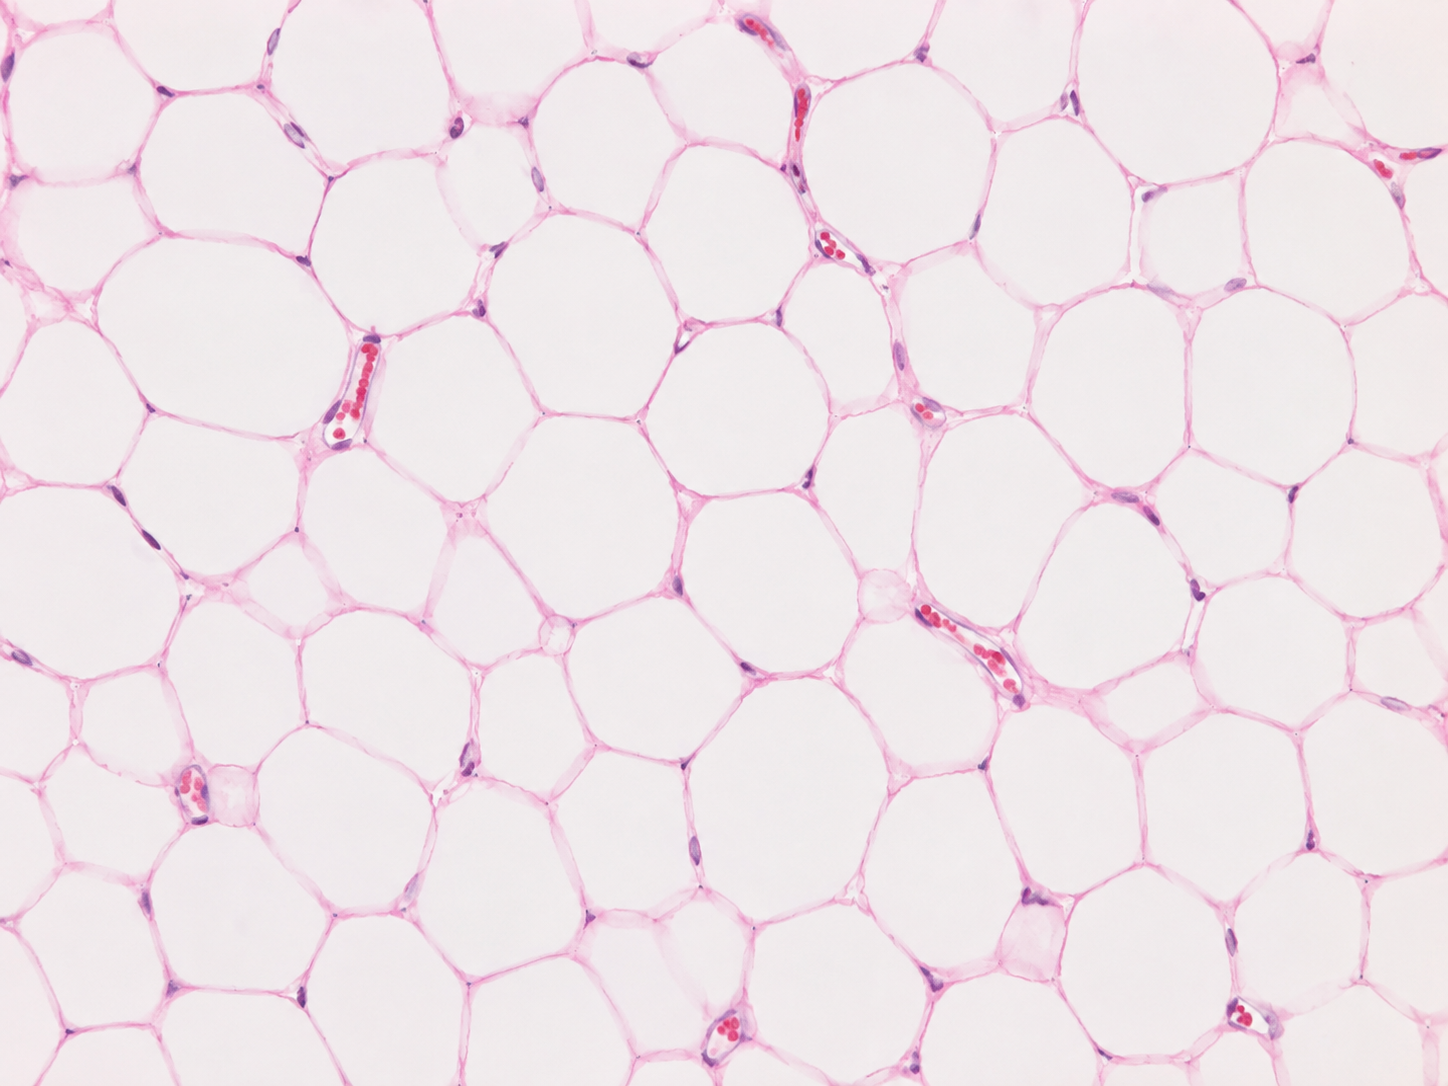
\includegraphics[width=0.5\linewidth]{images/book3/ai/b3-09-adipose-micrograph.png}

{\small \omterm{def:b1:body-plans-tissues:tissue}{Tecido} adiposo branco: cada \omterm{def:b1:cell-unit-of-life:cell}{célula} é uma gotícula de
\omterm{def:b1:lipids:triglyceride}{triglicerídeo}, de até \qty{100}{\micro m} de diâmetro, com o \omterm{def:b1:cell-unit-of-life:cell}{citoplasma}
e o núcleo espremidos num anel fino. Capilares correm entre as \omterm{def:b1:cell-unit-of-life:cell}{células}
para entregar e recolher \omterm{def:b1:lipids:fattyacid}{ácidos graxos}.}
\end{omfigure}

\begin{proposition}[A gordura é o estoque de energia mais denso]\label{prop:b1:lipids:energystore}
Oxidar \qty{1}{g} de \omterm{def:b1:lipids:triglyceride}{gordura} libera \qty{38}{kJ}, contra \qty{17}{kJ}
para \qty{1}{g} de carboidrato ou de proteína: os carbonos de um \omterm{def:b1:lipids:fattyacid}{ácido
graxo} são mais reduzidos (mais ligações C--H, menos C--O) e por isso
cedem mais elétrons ao oxigênio. Além disso a \omterm{def:b1:lipids:triglyceride}{gordura} é armazenada seca,
ao passo que o glicogênio liga cerca de \qty{3}{g} de água por grama:
\qty{1}{g} de glicogênio armazenado rende \qty{4}{kJ} por grama de massa
estocada, e a \omterm{def:b1:lipids:triglyceride}{gordura}, nove vezes mais. Um ser humano magro carrega
\qty{0.5}{kg} de glicogênio (a energia de um dia) e \qty{12}{kg} de
\omterm{def:b1:lipids:triglyceride}{gordura} (mais de um mês).
\end{proposition}

\begin{example}[Por que não armazenar tudo como gordura]\label{ex:b1:lipids:whyglycogen}
A \omterm{def:b1:lipids:triglyceride}{gordura} só pode ser queimada com oxigênio, devagar, e não pode ser
reconvertida em glicose nos animais
(\cref{ch:b1:biosyntheses-integration}); o encéfalo e as hemácias
precisam de glicose, e um músculo em disparada precisa dela mais rápido
do que a \omterm{def:b1:lipids:triglyceride}{gordura} consegue fornecer. O glicogênio é o estoque de glicose
rápido e sem oxigênio, para horas; a \omterm{def:b1:lipids:triglyceride}{gordura}, o estoque denso, para
semanas. Uma ave migratória, um arganaz em hibernação e um camelo são
\omterm{def:b1:lipids:triglyceride}{gordura}; as pernas de um velocista são glicogênio.
\end{example}

\begin{definition}[Ceras]\label{def:b1:lipids:wax}
As \emph{ceras}\index{cera} são ésteres de um \omterm{def:b1:lipids:fattyacid}{ácido graxo} com um álcool
de cadeia longa: sólidas, inteiramente hidrofóbicas, e usadas como
revestimentos --- a \omterm{def:b1:flowering-plant-organization:tissues}{cutícula} das \omterm{def:b1:flowering-plant-organization:organs}{folhas}
(\cref{ch:b1:flowering-plant-organization}), a superfície dos insetos, a
impermeabilização das penas e dos pelos, o favo das abelhas.
\end{definition}

\section{Lipídios de membrana e automontagem}

\begin{definition}[Lipídios anfifílicos]\label{def:b1:lipids:amphiphilic}
Os \omterm{def:b1:lipids:fattyacid}{lipídios} das membranas são
\emph{anfifílicos}\index{molécula anfifílica}: uma \emph{cabeça} \omterm{def:b1:water-small-molecules:water}{polar}
que a água solvata e uma ou duas \emph{caudas} apolares que ela exclui.
Os \emph{glicerofosfolipídios}\index{fosfolipídio} são o glicerol com
dois \omterm{def:b1:lipids:fattyacid}{ácidos graxos} e, no terceiro carbono, um fosfato ligado a um
pequeno álcool \omterm{def:b1:water-small-molecules:water}{polar} (colina, etanolamina, serina, inositol): a
fosfatidilcolina é o \omterm{def:b1:lipids:fattyacid}{lipídio} mais comum das membranas animais. Os
\emph{esfingolipídios}\index{esfingolipídio} são construídos sobre o
aminoálcool esfingosina, em vez do glicerol, com um \omterm{def:b1:lipids:fattyacid}{ácido graxo} e uma
cabeça de fosfocolina (a esfingomielina) ou de açúcares (os
glicolipídios), e são abundantes no folheto externo e nas bainhas
nervosas. Os \emph{esteróis}\index{esterol} --- o
\emph{colesterol}\index{colesterol} nos animais, esteróis aparentados
nas plantas e nos fungos --- são moléculas rígidas de quatro anéis, com
uma única hidroxila como cabeça, que se deitam entre as caudas dos
outros \omterm{def:b1:lipids:fattyacid}{lipídios}.
\end{definition}

\begin{proposition}[Automontagem]\label{prop:b1:lipids:selfassembly}
\index{automontagem}\index{micela}\index{lipossomo}
Em água, as \omterm{def:b1:lipids:amphiphilic}{moléculas anfifílicas} se montam espontaneamente de modo a
esconder as caudas e expor as cabeças. A forma da molécula decide a
estrutura: os \omterm{def:b1:lipids:fattyacid}{lipídios} de uma só cauda (\omterm{def:b1:lipids:fattyacid}{ácidos graxos}, detergentes), com
forma de cone, formam \emph{micelas} --- esferas de alguns nanômetros de
diâmetro com as caudas por dentro; os \omterm{def:b1:lipids:amphiphilic}{fosfolipídios} de duas caudas, com
forma de cilindro, formam \emph{bicamadas}, que se fecham sobre si
mesmas em \emph{lipossomos} (vesículas) para não deixar nenhuma borda
exposta. A montagem é movida pelo \omterm{prop:b1:water-small-molecules:properties}{efeito hidrofóbico}
(\cref{ch:b1:water-small-molecules}): ela não custa energia e não
precisa de enzima, e uma bicamada rasgada se refecha sozinha. As
membranas são lâminas que se autorreparam, crescem pela inserção de
\omterm{def:b1:lipids:fattyacid}{lipídios} novos e nunca se formam do nada: toda membrana vem de uma
membrana.
\end{proposition}
\begin{proof}[Evidências]
\omterm{def:b1:lipids:amphiphilic}{Fosfolipídio} seco disperso em água forma vesículas fechadas com paredes
em bicamada, visíveis ao \omterm{prop:b1:cell-unit-of-life:microscopes}{microscópio eletrônico} (Bangham, 1965); a
permeabilidade delas a íons e à água corresponde à das membranas
celulares, e elas podem ser carregadas com fármacos e fundidas com
\omterm{def:b1:cell-unit-of-life:cell}{células}. Acrescentar um detergente (de uma só cauda, em forma de cone)
dissolve a bicamada em micelas mistas; retirá-lo por diálise deixa a
bicamada se formar de novo.
\end{proof}

\begin{omfigure}
\begin{tikzpicture}[font=\footnotesize, line cap=round]
  % micelle: ring of heads with tails pointing inward
  \foreach \a in {0,30,...,330} {
    \fill[omDef!60] ({1.2*cos(\a)},{1.2*sin(\a)}) circle (0.14);
    \draw[omDef!70!black, thick] ({1.05*cos(\a)},{1.05*sin(\a)}) -- ({0.35*cos(\a)},{0.35*sin(\a)});
  }
  \node[anchor=north, align=center] at (0,-1.55) {micela: lipídios de\\ uma cauda (cones)};
  % bilayer segment
  \foreach \i in {0,...,9} {
    \fill[omDef!60] (3.2+0.36*\i,0.75) circle (0.13); \draw[omDef!70!black, thick] (3.14+0.36*\i,0.62) -- (3.14+0.36*\i,0.1) (3.26+0.36*\i,0.62) -- (3.26+0.36*\i,0.1);
    \fill[omDef!60] (3.2+0.36*\i,-0.75) circle (0.13); \draw[omDef!70!black, thick] (3.14+0.36*\i,-0.62) -- (3.14+0.36*\i,-0.1) (3.26+0.36*\i,-0.62) -- (3.26+0.36*\i,-0.1);
  }
  \node[anchor=north, align=center] at (4.85,-1.55) {bicamada: lipídios de\\ duas caudas (cilindros)};
  % liposome: two concentric rings of heads with tails between
  \foreach \a in {0,15,...,345} {
    \fill[omDef!60] ({9.3+1.45*cos(\a)},{1.45*sin(\a)}) circle (0.11);
    \draw[omDef!70!black, thick] ({9.3+1.33*cos(\a)},{1.33*sin(\a)}) -- ({9.3+1.0*cos(\a)},{1.0*sin(\a)});
    \fill[omDef!60] ({9.3+0.62*cos(\a)},{0.62*sin(\a)}) circle (0.10);
    \draw[omDef!70!black, thick] ({9.3+0.72*cos(\a)},{0.72*sin(\a)}) -- ({9.3+0.98*cos(\a)},{0.98*sin(\a)});
  }
  \node at (9.3,0) {água};
  \node[anchor=north, align=center] at (9.3,-1.55) {lipossomo: uma bicamada\\ fechada, sem bordas};
\end{tikzpicture}

{\small Três arranjos de \omterm{def:b1:lipids:fattyacid}{lipídios} \omterm{def:b1:lipids:amphiphilic}{anfifílicos} em água. As moléculas de
uma cauda, em forma de cone, se empacotam em micelas; os \omterm{def:b1:lipids:amphiphilic}{fosfolipídios}
cilíndricos de duas caudas formam uma bicamada, que se fecha numa
vesícula para esconder as bordas dela.}
\end{omfigure}

\begin{omfigure}
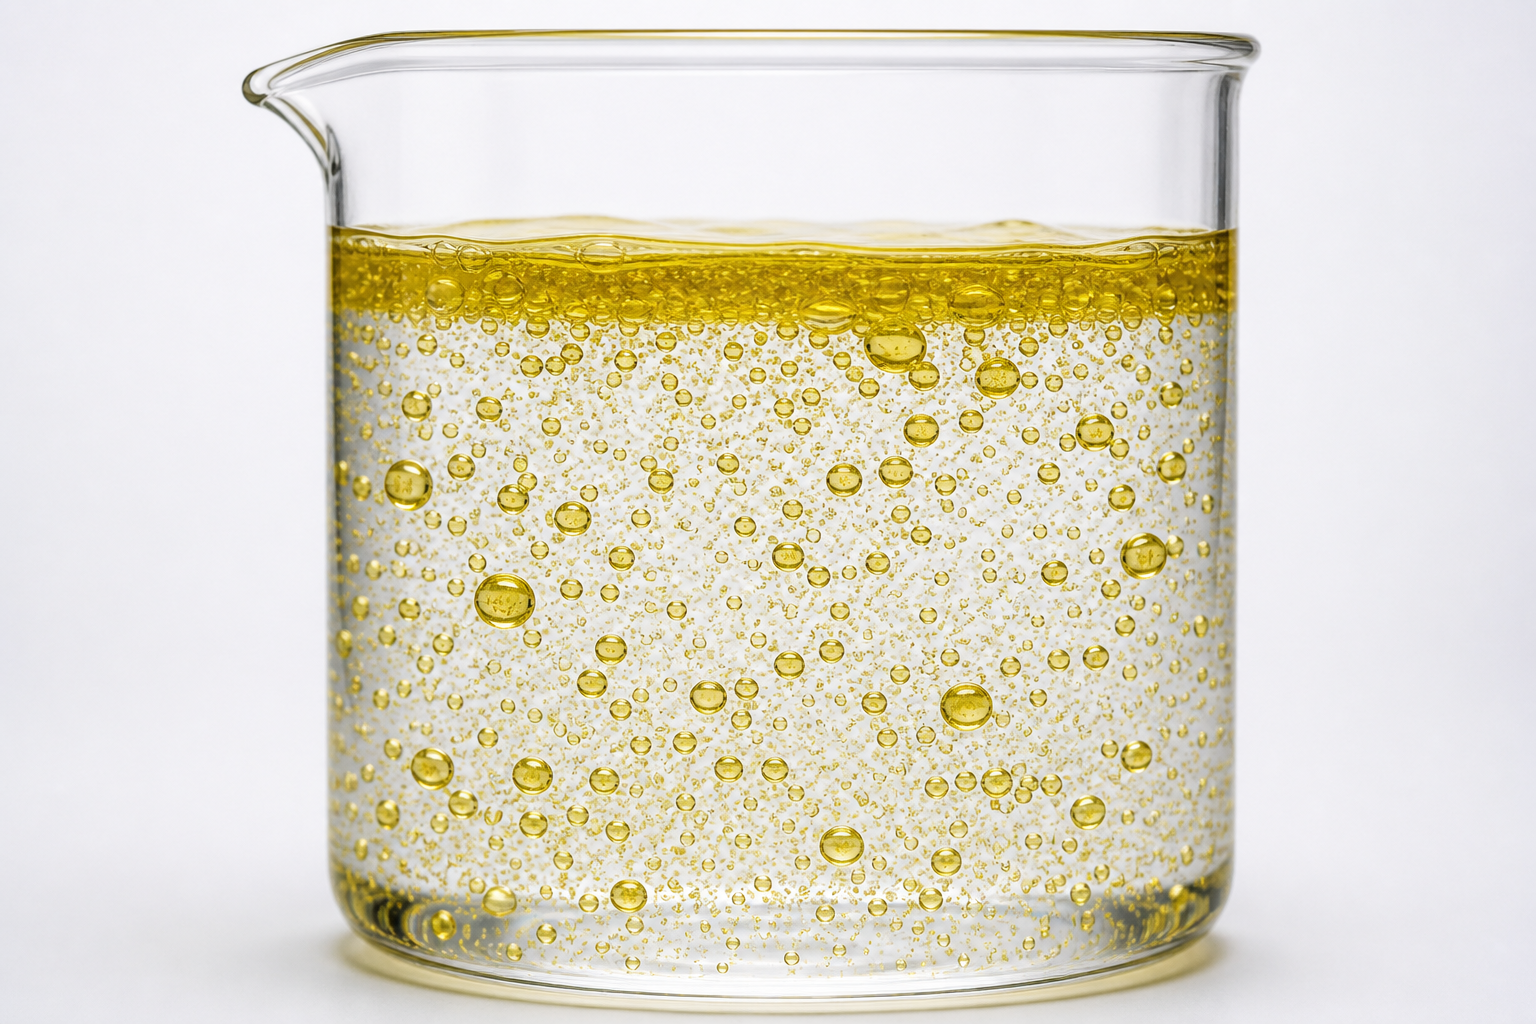
\includegraphics[width=0.5\linewidth]{images/book3/ai/b3-09-oil-water-emulsion.png}

{\small \omterm{def:b1:lipids:triglyceride}{Óleo} agitado em água: uma nuvem de gotículas que vão coalescer
em poucos minutos, a não ser que um anfifílico --- um detergente, um sal
biliar, um \omterm{def:b1:lipids:amphiphilic}{fosfolipídio} --- as recubra. A emulsificação é o que o
intestino faz com a \omterm{def:b1:lipids:triglyceride}{gordura} da dieta antes que as enzimas dele possam
alcançá-la.}
\end{omfigure}

\begin{example}[Sais biliares]\label{ex:b1:lipids:bile}
A \omterm{def:b1:lipids:triglyceride}{gordura} da dieta chega ao intestino como \omterm{def:b1:lipids:triglyceride}{óleo}; a lipase que a digere
só age na interface óleo--água. Os sais biliares, derivados \omterm{def:b1:lipids:amphiphilic}{anfifílicos}
do \omterm{def:b1:lipids:amphiphilic}{colesterol}, recobrem a \omterm{def:b1:lipids:triglyceride}{gordura} em gotículas de um micrômetro,
multiplicando a interface por mil, e depois levam, em micelas, os \omterm{def:b1:lipids:fattyacid}{ácidos
graxos} liberados até as \omterm{def:b1:cell-unit-of-life:cell}{células} absortivas
(\cref{ch:b1:digestion-absorption}). O sabão usa o mesmo truque.
\end{example}

\section{Fluidez da membrana}

\begin{definition}[Fluidez, transição de fase]\label{def:b1:lipids:fluidity}
Uma \omterm{def:b1:membranes-transport:membrane}{bicamada lipídica} tem uma
\emph{temperatura de transição de fase}\index{temperatura de transição de fase}
$T_m$: abaixo dela as cadeias ficam empacotadas num estado ordenado,
semelhante a um gel, em que os \omterm{def:b1:lipids:fattyacid}{lipídios} quase não se movem; acima dela
elas ficam desordenadas e a bicamada é um fluido bidimensional em que um
\omterm{def:b1:lipids:fattyacid}{lipídio} troca de lugar com a vizinha um milhão de vezes por segundo e
percorre o plano da membrana a \qty{1}{\micro m/s}. As \omterm{def:b1:cell-unit-of-life:cell}{células} mantêm as
membranas delas acima de $T_m$: a
\emph{fluidez}\index{fluidez da membrana} deixa as proteínas se
difundirem e girarem, as vesículas brotarem e se fundirem, e a bicamada
se refechar.
\end{definition}

\begin{proposition}[O que determina a fluidez]\label{prop:b1:lipids:fluidityfactors}
$T_m$ sobe com o comprimento das cadeias e cai com a insaturação delas,
como para os \omterm{def:b1:lipids:fattyacid}{ácidos graxos} livres; uma bicamada de cadeias C18:0 funde a
\qty{55}{\celsius}, e uma de cadeias C18:1 a \qty{-20}{\celsius}. O
\omterm{def:b1:lipids:amphiphilic}{colesterol}, inserido entre as caudas, tem efeito duplo: acima de $T_m$
os anéis rígidos dele restringem o movimento das cadeias e enrijecem a
membrana; abaixo de $T_m$ eles impedem que as cadeias se empacotem e a
impedem de congelar. Ele alarga a transição, tornando-a uma mudança
gradual, e mantém a \omterm{def:b1:lipids:fluidity}{fluidez} quase constante numa ampla faixa de
temperatura --- um \omterm{def:b1:water-small-molecules:buffer}{tampão} de \omterm{def:b1:lipids:fluidity}{fluidez}. As membranas plasmáticas animais
chegam a um \omterm{def:b1:lipids:amphiphilic}{colesterol} para cada \omterm{def:b1:lipids:amphiphilic}{fosfolipídio}.
\end{proposition}

\begin{omfigure}
\begin{tikzpicture}
\begin{axis}[
  width=0.86\linewidth, height=6.0cm,
  axis x line=bottom, axis y line=left,
  xmin=-20, xmax=60, ymin=0, ymax=1.15,
  xlabel={temperatura (\unit{\celsius})}, ylabel={fluidez (relativa)},
  xlabel style={font=\small, at={(axis description cs:0.5,-0.12)}, anchor=north},
  ylabel style={font=\small},
  tick label style={font=\small}, xtick={-20,0,20,40,60}, ytick={0,0.5,1},
  legend style={font=\small, at={(0.03,0.97)}, anchor=north west, draw=none},
  clip=false,
]
\addplot[very thick, omDef, domain=-20:60, samples=120] {1/(1+exp(-(x-41)/1.5))};
\addlegendentry{cadeias C16 saturadas, sem colesterol}
\addplot[very thick, omProp, domain=-20:60, samples=120] {1/(1+exp(-(x+5)/1.5))};
\addlegendentry{uma ligação dupla \emph{cis} por lipídio}
\addplot[very thick, omThm, domain=-20:60, samples=120] {0.15+0.7/(1+exp(-(x-20)/12))};
\addlegendentry{cadeias saturadas com \qty{30}{\%} de colesterol}
\draw[dashed, gray] (axis cs:37,0) -- (axis cs:37,1.05);
\node[font=\scriptsize, anchor=south] at (axis cs:37,1.06) {\qty{37}{\celsius}};
\end{axis}
\end{tikzpicture}

{\small \omterm{def:b1:lipids:fluidity}{Fluidez} em função da temperatura para três bicamadas. As cadeias
saturadas congelam bruscamente perto de \qty{40}{\celsius}; uma ligação
dupla por \omterm{def:b1:lipids:fattyacid}{lipídio} baixa a transição abaixo de zero; o \omterm{def:b1:lipids:amphiphilic}{colesterol} suaviza
a transição, tornando-a uma rampa branda, e mantém a membrana nem sólida
nem fluida demais em toda a faixa fisiológica.}
\end{omfigure}

\begin{proposition}[Adaptação homeoviscosa]\label{prop:b1:lipids:homeoviscous}
\index{adaptação homeoviscosa}
Os \omterm{def:b1:organism-environment:organism}{organismos} que não conseguem regular a própria temperatura ajustam a
composição das membranas para manter a \omterm{def:b1:lipids:fluidity}{fluidez} constante: quando a
temperatura cai, eles substituem \omterm{def:b1:lipids:fattyacid}{ácidos graxos saturados} por
insaturados e cadeias longas por mais curtas, e o inverso quando ela
sobe.
\end{proposition}
\begin{proof}[Evidências]
A \emph{E. coli} cultivada a \qty{10}{\celsius} tem o dobro da proporção
de \omterm{def:b1:lipids:fattyacid}{ácidos graxos insaturados} da mesma linhagem cultivada a
\qty{40}{\celsius}, e as membranas das duas culturas, medidas pela
mobilidade de uma sonda, são igualmente fluidas nas respectivas
temperaturas de cultivo. Trutas aclimatadas a \qty{5}{\celsius} carregam
mais ácidos poli-insaturados nos \omterm{def:b1:lipids:fattyacid}{lipídios} de membrana que trutas a
\qty{20}{\celsius}; a \omterm{def:b1:lipids:triglyceride}{gordura} das pernas das renas, junto da neve, é
mais insaturada que a \omterm{def:b1:lipids:triglyceride}{gordura} do tronco. As plantas que sobrevivem à
geada enriquecem as membranas em \omterm{def:b1:lipids:fattyacid}{lipídios} insaturados no outono, e os
mutantes incapazes de fazê-lo morrem quando esfria.
\end{proof}

\begin{example}[Manteiga, azeite, óleo de peixe]\label{ex:b1:lipids:kitchen}
A manteiga (\qty{65}{\%} de saturados) é sólida na geladeira e mole à
temperatura ambiente; o azeite (\qty{75}{\%} de ácido oleico) é líquido
à temperatura ambiente e turva na geladeira; o \omterm{def:b1:lipids:triglyceride}{óleo} de peixe, rico em
ácidos ômega-3 com cinco e seis ligações duplas, permanece líquido a
\qty{-20}{\celsius}, que é o que as membranas de um bacalhau precisam no
Atlântico Norte.
\end{example}

\section{Esteróis, pigmentos e sinais}

\begin{definition}[Esteroides, isoprenoides]\label{def:b1:lipids:steroids}
Os \emph{esteroides}\index{esteroide} compartilham os quatro anéis
fundidos do \omterm{def:b1:lipids:amphiphilic}{colesterol}: o próprio \omterm{def:b1:lipids:amphiphilic}{colesterol} (membranas, e precursor dos
demais), os sais biliares, a vitamina D e os hormônios esteroides ---
cortisol, aldosterona, hormônios sexuais --- moléculas pequenas e
hidrofóbicas que atravessam membranas livremente e agem sobre receptores
dentro da \omterm{def:b1:cell-unit-of-life:cell}{célula}. Os \emph{isoprenoides}\index{isoprenoide} (terpenos)
são cadeias e anéis de unidades de isopreno de cinco carbonos: os
\emph{carotenoides} que dão cor às cenouras e protegem os \omterm{def:b1:eukaryotic-cell:plastid}{cloroplastos}
(\cref{ch:b1:photosynthesis}), a cadeia lateral da clorofila, as
quinonas das cadeias de transporte de elétrons, a borracha e as
vitaminas lipossolúveis A, E e K.
\end{definition}

\begin{proposition}[O que os lipídios fazem]\label{prop:b1:lipids:functions}
Armazenamento de energia (\omterm{def:b1:lipids:triglyceride}{triglicerídeos}); membranas (\omterm{def:b1:lipids:amphiphilic}{fosfolipídios},
\omterm{def:b1:lipids:amphiphilic}{esfingolipídios}, \omterm{def:b1:lipids:amphiphilic}{esteróis}); isolamento e impermeabilização (\omterm{def:b1:lipids:triglyceride}{gordura},
\omterm{def:b1:lipids:wax}{ceras}); absorção de luz e proteção (carotenoides); transporte de
elétrons (quinonas); sinalização entre \omterm{def:b1:cell-unit-of-life:cell}{células} (hormônios \omterm{def:b1:lipids:steroids}{esteroides},
prostaglandinas) e dentro delas (\omterm{def:b1:lipids:amphiphilic}{fosfolipídios} de inositol,
diacilglicerol); vitaminas. Uma única propriedade --- a insolubilidade
em água --- está por trás de todas elas: um \omterm{def:b1:lipids:fattyacid}{lipídio} fica onde é posto,
numa gotícula, numa película ou numa membrana, ou atravessa uma membrana
sem carreador.
\end{proposition}

\begin{example}[Um hormônio que não precisa de receptor na superfície]\label{ex:b1:lipids:steroidhormone}
O cortisol, secretado pela glândula adrenal, viaja no sangue ligado a
uma proteína carreadora, a deixa numa célula-alvo, se dissolve através
da membrana plasmática em segundos, e se liga a um receptor do \omterm{def:b1:eukaryotic-cell:organelle}{citosol}
que então entra no núcleo e liga genes
(\cref{ch:b1:expression-control}). Um hormônio proteico como a insulina,
solúvel em água e grande demais para atravessar, precisa se ligar a um
receptor do lado de fora e ter a mensagem dele retransmitida para
dentro. A química do mensageiro decide a rota da mensagem.
\end{example}

\section{Exercícios}

\begin{exercise}[$\star$]\label{exo:b1:lipids:1}
Defina um \omterm{def:b1:lipids:fattyacid}{lipídio} e explique por que a definição é por propriedade, e
não por estrutura.
\end{exercise}

\begin{exercise}[$\star$]\label{exo:b1:lipids:2}
Escreva a notação do ácido linoleico (18 carbonos, ligações duplas
depois dos carbonos 9 e 12) e diga se ele é um ácido ômega-3 ou ômega-6.
\end{exercise}

\begin{exercise}[$\star$]\label{exo:b1:lipids:3}
Por que um \omterm{def:b1:lipids:triglyceride}{triglicerídeo} forma gotículas enquanto um \omterm{def:b1:lipids:amphiphilic}{fosfolipídio} forma
bicamadas? Que diferença estrutural é responsável por isso?
\end{exercise}

\begin{exercise}[$\star$]\label{exo:b1:lipids:4}
A partir da figura da \omterm{def:b1:lipids:fluidity}{fluidez}, em que temperatura cada uma das três
bicamadas está na metade da transição dela? Qual você esperaria numa
bactéria que vive a \qty{10}{\celsius}?
\end{exercise}

\begin{exercise}[$\star\star$]\label{exo:b1:lipids:5}
Uma pessoa armazena \qty{15}{kg} de \omterm{def:b1:lipids:triglyceride}{gordura}. Calcule a energia que ela
contém, o número de dias em que ela sustentaria um gasto de repouso de
\qty{8}{MJ/d}, e a massa de glicogênio hidratado que conteria a mesma
energia.
\end{exercise}

\begin{exercise}[$\star\star$]\label{exo:b1:lipids:6}
Ordene por ponto de fusão: C14:0, C18:0, C18:1, C18:3, C22:0, e
justifique cada passo da ordenação.
\end{exercise}

\begin{exercise}[$\star\star$]\label{exo:b1:lipids:7}
Uma hemácia tem superfície de \qty{140}{\micro m^2}; uma cabeça de
\omterm{def:b1:lipids:amphiphilic}{fosfolipídio} ocupa \qty{0.6}{nm^2}. Calcule o número de moléculas de
\omterm{def:b1:lipids:amphiphilic}{fosfolipídio} da membrana (os dois folhetos) e, a \qty{750}{g/mol}, a
massa total delas em picogramas.
\end{exercise}

\begin{exercise}[$\star\star$]\label{exo:b1:lipids:8}
\qty{1}{g} de azeite (densidade \qty{0.9}{g/mL}) é emulsificado em
gotículas de \qty{1}{\micro m} de diâmetro. Calcule a área total da
interface. Repita para uma gota única. Por que a lipase pancreática
precisa da emulsão?
\end{exercise}

\begin{exercise}[$\star\star$]\label{exo:b1:lipids:9}
Explique os dois efeitos opostos do \omterm{def:b1:lipids:amphiphilic}{colesterol} sobre a \omterm{def:b1:lipids:fluidity}{fluidez da
membrana} e por que uma membrana com \omterm{def:b1:lipids:amphiphilic}{colesterol} não tem transição
brusca.
\end{exercise}

\begin{exercise}[$\star\star\star$]\label{exo:b1:lipids:10}
Uma planta mutante não consegue fabricar \omterm{def:b1:lipids:fattyacid}{ácidos graxos insaturados}.
Preveja as membranas dela a \qty{25}{\celsius} e a \qty{5}{\celsius}, o
que acontece com as \omterm{def:b1:cell-unit-of-life:cell}{células} dela numa noite fria, e por que o tipo
selvagem sobrevive.
\end{exercise}

\begin{exercise}[$\star\star\star$]\label{exo:b1:lipids:11}
A \omterm{def:b1:lipids:triglyceride}{gordura} dá \qty{1.07}{g} de água por grama oxidado (o glicogênio
\qty{0.56}{g}, a proteína \qty{0.4}{g}). Calcule a água produzida por um
camelo que oxida \qty{1}{kg} de \omterm{def:b1:lipids:triglyceride}{gordura}. O oxigênio necessário é de
\qty{2}{L} por grama de \omterm{def:b1:lipids:triglyceride}{gordura}; respirá-lo no ar seco do deserto custa
cerca de \qty{0.03}{g} de água por litro de ar ventilado, com
\qty{5}{\%} de extração de oxigênio. Calcule a água perdida na
respiração e diga se a corcova é um estoque de água.
\end{exercise}

\begin{exercise}[$\star\star\star$]\label{exo:b1:lipids:12}
``Uma membrana se monta sozinha, mas uma \omterm{def:b1:cell-unit-of-life:cell}{célula} não consegue fabricar
uma membrana do nada.'' Concilie as duas metades da frase em um
parágrafo, usando o \omterm{prop:b1:water-small-molecules:properties}{efeito hidrofóbico}, o crescimento das membranas por
inserção, e a continuidade das membranas através da divisão celular.
\end{exercise}

\section{Problema: Água fria e gordura de deserto}

\begin{problem}[{Problema de fim de semana --- as membranas de uma truta
num riacho de montanha e a corcova de um camelo no deserto:
insaturação, temperaturas de transição, densidade de energia e água
metabólica, terminando na massa que armazenar gordura em vez de
glicogênio poupa}]
\label{pb:b1:lipids:1}
A Parte I trata de uma truta cujos \omterm{def:b1:lipids:amphiphilic}{fosfolipídios} de membrana carregam
cadeias de C16:0, C18:1 e C22:6 (um ácido ômega-3 com seis ligações
duplas). A Parte II trata de um dromedário de \qty{500}{kg} com uma
corcova de \qty{30}{kg} de \omterm{def:b1:lipids:triglyceride}{triglicerídeo}, atravessando um deserto a uma
\omterm{def:b1:organism-environment:allometry}{taxa metabólica} de \qty{60}{MJ/d}. Energia: \omterm{def:b1:lipids:triglyceride}{gordura} \qty{38}{kJ/g},
glicogênio \qty{17}{kJ/g} a seco, armazenado com \qty{3}{g} de água por
grama. Água metabólica: \qty{1.07}{g/g} de \omterm{def:b1:lipids:triglyceride}{gordura}. Oxigênio:
\qty{2.0}{L} por grama de \omterm{def:b1:lipids:triglyceride}{gordura}; o ar tem \qty{21}{\%} de oxigênio; o
camelo extrai \qty{5}{\%} do oxigênio que respira; o ar exalado carrega
\qty{30}{g/m^3} de água a mais que o ar do deserto inalado.

\medskip
\noindent\textbf{Parte I --- A truta.}
As trutas aclimatadas a \qty{20}{\celsius} têm cadeias de membrana com
\qty{40}{\%} de C16:0, \qty{45}{\%} de C18:1 e \qty{15}{\%} de C22:6; as
trutas a \qty{5}{\celsius}, \qty{25}{\%}, \qty{40}{\%} e \qty{35}{\%}.
\begin{enumerate}
  \item Escreva a notação dos três ácidos e conte as ligações duplas por
        cadeia em cada um.
  \item Calcule o número médio de ligações duplas por cadeia em cada
        temperatura.
  \item Explique, a partir do empacotamento das cadeias, por que a
        mudança baixa a temperatura de transição da membrana.
  \item O $T_m$ de uma bicamada cai cerca de \qty{20}{\celsius} para
        cada \qty{0.5}{} ligação dupla a mais por cadeia, em média.
        Estime o deslocamento de $T_m$ entre as duas trutas.
  \item A membrana da truta de água morna é fluida a \qty{20}{\celsius},
        mas gelificaria a \qty{5}{\celsius}. O que aconteceria com as
        proteínas de transporte, com as bombas e com a condução nervosa
        dela numa noite fria repentina?
  \item A adaptação leva dias. Cite as enzimas de que a truta precisa
        fabricar mais, e onde na \omterm{def:b1:cell-unit-of-life:cell}{célula} elas agem (\cref{ch:b1:eukaryotic-cell}).
  \item O \omterm{def:b1:lipids:amphiphilic}{colesterol} está a uma molécula por dois \omterm{def:b1:lipids:amphiphilic}{fosfolipídios} nas duas
        trutas. Explique o que ele contribui em cada caso.
\end{enumerate}

\medskip
\noindent\textbf{Parte II --- A energia do camelo.}
\begin{enumerate}[resume]
  \item Calcule a energia armazenada na corcova.
  \item Para quantos dias de travessia ela basta?
  \item Calcule a massa de glicogênio seco que contém a mesma energia, e
        a massa de glicogênio hidratado.
  \item Calcule a massa poupada por armazenar \omterm{def:b1:lipids:triglyceride}{gordura} em vez de
        glicogênio, e expresse-a como fração da massa corporal do
        camelo.
  \item A \omterm{def:b1:lipids:triglyceride}{gordura} é armazenada numa corcova, e não espalhada sob a pele.
        Proponha uma razão, a partir do balanço térmico do
        \cref{ch:b1:mammal-organization}.
\end{enumerate}

\medskip
\noindent\textbf{Parte III --- A corcova é um estoque de água?}
\begin{enumerate}[resume]
  \item Calcule a água metabólica produzida ao oxidar a corcova
        inteira.
  \item Calcule o oxigênio necessário, em litros.
  \item Calcule o volume de ar que o camelo precisa ventilar para
        obtê-lo.
  \item Calcule a água perdida ao exalar esse ar.
  \item Compare a água ganha com a água perdida e conclua.
  \item Em vez de transpirar, o camelo deixa a temperatura corporal
        subir \qty{6}{\celsius} durante o dia e esfriar à noite. Calcule
        o calor que ele armazena assim (capacidade térmica
        \qty{3.5}{kJ.kg^{-1}.K^{-1}}) e a água que evaporar o mesmo
        calor custaria (\qty{2.4}{kJ/g}).
  \item Um camelo pode perder \qty{25}{\%} da água corporal e
        sobreviver, e as hemácias dele incham até o dobro do volume sem
        estourar quando ele bebe \qty{100}{L} em dez minutos. Relacione
        a segunda propriedade com as membranas do
        \cref{ch:b1:membranes-transport}.
\end{enumerate}

\medskip
\noindent\textbf{Parte IV --- A aritmética da bicamada.}
Uma cabeça de \omterm{def:b1:lipids:amphiphilic}{fosfolipídio} ocupa \qty{0.65}{nm^2}; uma bicamada tem
\qty{5}{nm} de espessura; as hemácias do camelo têm superfície de
\qty{80}{\micro m^2} e são $\num{8e12}$ por litro de sangue.
\begin{enumerate}[resume]
  \item Calcule o número de \omterm{def:b1:lipids:amphiphilic}{fosfolipídios} de uma membrana de hemácia.
  \item Calcule o número em todas as hemácias de \qty{40}{L} de sangue.
  \item A \qty{750}{g/mol}, calcule a massa desse \omterm{def:b1:lipids:fattyacid}{lipídio} em gramas.
  \item Um \omterm{def:b1:lipids:amphiphilic}{fosfolipídio} passa espontaneamente de um folheto ao outro
        cerca de uma vez por semana, mas se difunde lateralmente
        \qty{1}{\micro m} em um segundo. Explique os dois números a
        partir do \omterm{prop:b1:water-small-molecules:properties}{efeito hidrofóbico}.
  \item Explique por que, dada a taxa de passagem entre folhetos, os
        dois folhetos de uma membrana podem permanecer diferentes em
        composição por toda a vida de uma \omterm{def:b1:cell-unit-of-life:cell}{célula}.
  \item Enuncie o resultado: a massa que o camelo poupa ao carregar
        \qty{30}{kg} de \omterm{def:b1:lipids:triglyceride}{gordura} em vez do glicogênio de igual energia, e
        o veredicto sobre a corcova como estoque de água.
\end{enumerate}
\end{problem}
